
%% ==================================================================================================
%%
\documentclass[12pt]{book}
\usepackage{amsfonts}
\usepackage{amsmath}
\usepackage{amssymb}
\usepackage{graphicx}
\usepackage{hyperref}
\usepackage{float}
\usepackage{verbatim}
\usepackage{xlop} %% for multiplication https://tex.stackexchange.com/questions/11702/how-to-present-a-vertical-multiplication-addition
\usepackage{listings} %% to format generic computer code
\usepackage{lmodern} % for bold teletype font
\usepackage{minted} % colour Java code

\usepackage{tasks}
%\NewTasks[style=enumerate,counter-format=tsk[A].,label-width=3ex]{choice}[\item](4)

%% =======   set page margins    =======
\setlength{\textheight}{10in}
\setlength{\textwidth}{7.4in}
\setlength{\topmargin}{-0.75in}
\setlength{\oddsidemargin}{-0.5in}
\setlength{\evensidemargin}{-0.5in}
\setlength{\parskip}{0.15in}
\setlength{\parindent}{0in}

%%  for European long division
% https://tex.stackexchange.com/questions/432435/how-to-set-up-european-french-style-long-division-in-tex
\newcommand\frdiv[5]{%
    \[
    \renewcommand\arraystretch{1.5}
    \begin{array}{l| l}
    #1 & #2 \\
    \cline{2-2}
    #3 & #4 \\
    \cline{1-1}
    #5 & \\
    \end{array}
    \]
}

%%  for European long division


%% ==================================================================================================

\begin{document}

\newcommand{\reporttitle}{Assignment 3}
\newcommand{\reportauthorOne}{Kien Do}
\newcommand{\cidOne}{300163370}
\input{titlePage/titlepage.txt}



%% ==================================================================================================

%%%%%%%%%%%% PROBLEMS START HERE

\begin{enumerate}
    %% ============================   New Item   ============================
    \item \textbf{Answer}
    
    This is a z-test question for one mean (where $\sigma$ is known).
    
    \begin{enumerate}
        \item
        
        We are given the following information,
        $$ H_0: \mu = 4.5, \,\, H_a: \mu \neq 4.5, \,\, \alpha = 0.05$$
        $$\bar{X} = 3.96, \,\, \sigma = 1.5, n = 25$$
        % https://www.youtube.com/watch?v=pGv13jvnjKc&list=PLvxOuBpazmsNo893xlpXNfMzVpRBjDH67&index=2
        Since $\sigma$ is given, we can use the Z test.
        % version 2: p-value, z-test
        \begin{align*}
            Z &= \dfrac{\bar{X} - \mu_0}{\sigma_{\bar{X}}}\\
            Z &= \dfrac{\bar{X} - \mu_0}{\sigma / \sqrt{n}}\\
            Z &= \dfrac{3.96 - 4.5}{1.5 / \sqrt{25}}\\
            Z &= -1.8
        \end{align*}
        From the Normal Probability Table, we have that the area (p-value) under -1.8 and 1.8 on both tail ends (left tail end, multiplied by 2) is,
        $$p = 2 \times 0.0359 = 0.0718$$
        If $p \leq \alpha$, the evidence against the null hypothesis is significant and we would reject $H_0$. However, since $0.0718 > 0.05$, we have that the evidence against the null hypothesis, $H_0$, is not significant at the 0.05 level of significance.\\
        
        $\therefore$ The data does not provide strong evidence to the manager’s concern.
        
        \item
        
        We are given the following information,
        $$ H_0: \mu = 4.5, \,\, H_a: \mu < 4.5, \,\, \alpha = 0.05$$
        $$\bar{X} = 3.96, \,\, \sigma = 1.5, n = 25$$
        % https://www.youtube.com/watch?v=pGv13jvnjKc&list=PLvxOuBpazmsNo893xlpXNfMzVpRBjDH67&index=2
        Since $\sigma$ is given, we can use the Z test.
        \begin{align*}
            Z &= \dfrac{\bar{X} - \mu_0}{\sigma / \sqrt{n}}\\
            Z &= \dfrac{3.96 - 4.5}{1.5 / \sqrt{25}}\\
            Z &= -1.8
        \end{align*}
        Find the p-value (left tail end) from the Normal Probability Table,
        \begin{align*}
            P(Z < -1.8) &= 0.0359
        \end{align*}
        Since $p \leq a$, that is, $0.0359 \leq 0.05$, the evidence against the null hypothesis is significant.\\
        
        $\therefore$ The data does provide strong evidence to the manager's concern.
        
    \end{enumerate}
    
    \newpage
    
    %% ============================   New Item   ============================
    \item \textbf{Answer}
    
    %https://www.youtube.com/watch?v=m6sGjWz2CPg&list=PLvxOuBpazmsNo893xlpXNfMzVpRBjDH67&index=4
    This is a t-test question for one mean (where $\sigma_{\bar{X}}$ is not known).\\
    
    Find $\bar{X}$.
    $$\bar{X} = \dfrac{\sum_{i=0}^{n} x_i}{n} = 2.5$$
    
    Find the sample standard deviation, $S$, from the 12 water specimens.
    $$S = \sqrt{\dfrac{1}{n-1} \left(\sum x_{i}^2 - \dfrac{1}{n} \left(\sum x_{i}\right)^2\right)} = 0.286$$
    Determine the test statistic, $t_0$.
    \begin{align*}
            t_0 &= \dfrac{\bar{X} - \mu_0}{S / \sqrt{n}}\\
            t_0 &= \dfrac{2.5 - 2.25}{0.286 / \sqrt{12}}\\
            t_0 &= 3.028
    \end{align*}
    We can determine that the p-value is $$p = P(\bar{X} > 2.25) \quad t_0 > 3.028$$
    where T follows the t-distribution with $v = n - 1 = 11$ degrees of freedom. From the t-distribution table, we see that, for $v = 11$,\\
    
    $\qquad \qquad \qquad P(T(11) \geq 2.879) \approx 0.0075 \qquad$ and $\qquad P(T(11) \leq 3.106) \approx 0.005$
    
    Hence, the corresponding p-value is somewhere between the interval $(0.005, 0.0075)$, 
    \begin{align*}
        \text{p-value} &\stackrel{?}{=} a\\
        (0.005, 0.0075) &\geq 0.005
    \end{align*}
    which is not strong evidence against $H_0:\mu = 2.25$, because p-value $\leq a$ is not true.\\
    
    $\therefore$ We do not reject the null hypothesis, $H_0$.
        
    \newpage
    
    %% ============================   New Item   ============================
    \item \textbf{Answer}
    
\begin{minted}[breaklines,frame=single]{R}
> weight <- c(91, 121, 82, 90, 110, 91, 108, 114, 107, 115, 98, 87, 89)
> height <- c(191, 209, 191, 196, 199, 191, 201, 206, 194, 209, 204, 188, 194)
> # a) =======================================================================
> t.test(weight, mu = 90, alternative = "greater")

        One Sample t-test

data:  weight
t = 2.8905, df = 12, p-value = 0.006782
alternative hypothesis: true mean is greater than 90
95 percent confidence interval:
 93.92247      Inf
sample estimates:
mean of x 
 100.2308 

> # b) =======================================================================
> t.test(height, mu = 202, alternative = "less")

        One Sample t-test

data:  height
t = -2.0209, df = 12, p-value = 0.03309
alternative hypothesis: true mean is less than 202
95 percent confidence interval:
     -Inf 201.5187
sample estimates:
mean of x 
 197.9231 

> # c) =======================================================================
> cor(weight, height)
[1] 0.8512498
> # d) =======================================================================
> plot(weight, height)
> data <- data.frame(weight, height)
> regression_line <- lm(height~weight, data = data)
> abline(regression_line)
\end{minted}
\newpage
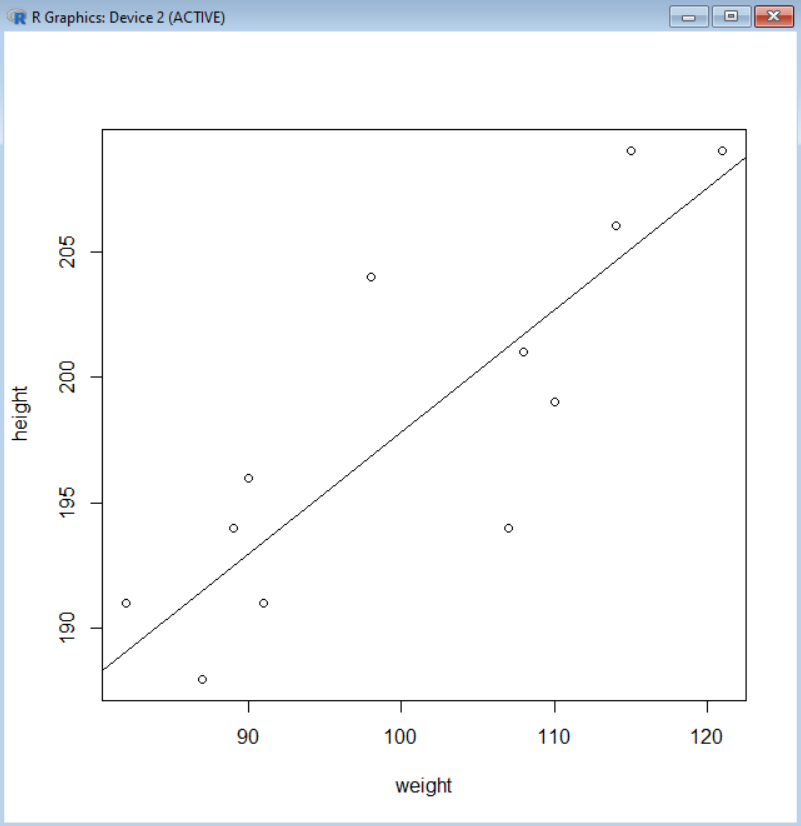
\includegraphics[scale=0.8]{A3_Q3_scatterplot.png}
    
    \newpage
    
    %% ============================   New Item   ============================
    \item \textbf{Answer}
    
    \begin{enumerate}
    % ========== part a ==========
        \item Compute the sample correlation coefficient of $x$ and $y$.\\
        
        Use the formula to find the sample coefficient of a correlation.
        $$r_{xy} = \dfrac{\sum (x_i - \bar{x}) (y_i - \bar{y})}{\sqrt{\sum \left(x_i - \bar{x}\right)^2} \sqrt{\sum \left(y_i - \bar{y}\right)^2}} = \dfrac{S_{xy}}{\sqrt{S_{xx} S_{yy}}}$$
        First, calculate the mean of $x$,
        \begin{align*}
            \bar{x} &= \dfrac{5 + 12 + 26 + 42 + 60 + 79}{6}\\
            \bar{x} &= 37.33
        \end{align*}
        and the mean of $y$,
        \begin{align*}
            \bar{y} &= \dfrac{120 + 132 + 139 + 169 + 201 + 220}{6}\\
            \bar{y} &= 163.5
        \end{align*}
        % Calculate the sample standard deviation of $x$, $S_x$,
        % \begin{align*}
        %     S_x &= \sqrt{\dfrac{1}{n-1} \sum^{n}_{i=1}\left( X_i - \bar{X} \right)^2}\\
        %     S_x &= \sqrt{\dfrac{1}{6-1} \sum^{n}_{i=1}\left( X_i - 37.33 \right)^2}\\
        %     S_x &= 28.59
        % \end{align*}
        % and the sample standard deviation of $y$, $S_y$,
        % \begin{align*}
        %     S_y &= \sqrt{\dfrac{1}{6-1} \sum^{n}_{i=1}\left( X_i - 163.5 \right)^2}\\
        %     S_y &= 40.28
        % \end{align*}
        Calculate $S_{xy}$,
        \begin{align*}
            S_{xy} &= \sum_{i=0}^n (x_i - \bar{x}) (y_i - \bar{y})\\
            S_{xy} &= 5712
        \end{align*}
        Calculate $S_{xx}$,
        \begin{align*}
            S_{xx} &= \sum_{i=0}^n \left(x_i - \bar{x}\right)^2\\
            S_{xx} &= 4087.333
        \end{align*}
        Calculate $S_{yy}$,
        \begin{align*}
            S_{yy} &= \sum_{i=0}^n \left(y_i - \bar{y}\right)^2\\
            S_{yy} &= 8113.5
        \end{align*}
        Calculate $r_{xy}$,
        \begin{align*}
            r_{xy} &= \dfrac{S_{xy}}{\sqrt{S_{xx} S_{yy}}}\\
            r_{xy} &= \dfrac{5712}{\sqrt{4087.333 \times 8113.5}}\\
            r_{xy} &= 0.9918912
        \end{align*}
        
        \newpage
        
        % ========== part b ==========
        \item Find the estimated regression line $y = b_0 + b_1x$.\\
        
        We know, from part a, that
        \begin{align*}
            \bar{x} &= 37.33\\
            \bar{y} &= 163.5\\
            S_{xy} &= 5712\\
            S_{xx} &= 4087.333\\
            S_{yy} &= 8113.5
        \end{align*}
        So, we need to find $\hat{\beta}_0$ and $\hat{\beta}_1$ in the regression line in the form $\bar{Y} = \hat{\beta}_0 + \hat{\beta}_1 \bar{X}$.\\
        
        Find $\hat{\beta}_1$.
        \begin{align*}
            \hat{\beta}_1 &= \dfrac{S_{xy}}{S_{xx}}\\
            \hat{\beta}_1 &= \dfrac{5712}{4087.33}\\
            \hat{\beta}_1 &= 1.397
        \end{align*}
        Find $\hat{\beta}_0$.
        \begin{align*}
            \hat{\beta}_0 &= \bar{y} - \hat{\beta}_1 \bar{x}\\
            \hat{\beta}_0 &= 163.5 - (1.397)(37.33)\\
            \hat{\beta}_0 &= 111.327
        \end{align*}
        Therefore, the regression line is,
        $$y = 111.327 + 1.397x$$
        
        % ========== part c ==========
        \item Compute the estimated standard errors.
        \begin{align*}
            SE &= S_{yy} - b_1 S_{xy}\\
            SE &= 8113.5 - (1.397)(5712)\\
            SE &= 131.04
        \end{align*}
        Find the variance, $\sigma_2$,
        \begin{align*}
            \sigma^2 &= \dfrac{SE}{n-2}\\
            \sigma^2 &= \dfrac{131.04}{6 - 2}\\
            \sigma^2 &= 32.76
        \end{align*}
        Find standard error of $b_0$,
        \begin{align*}
            SE_{b_0} &= \sqrt{\sigma^2 \left(\dfrac{1}{n} + \dfrac{\bar{x}^2}{S_{xx}}\right)}\\
            SE_{b_0} &= \sqrt{32.26 \left(\dfrac{1}{6} + \dfrac{(37.33)^2}{4087.33}\right)}\\
            SE_{b_0} &= 4.078
        \end{align*}
        Find standard error of $b_1$,
        \begin{align*}
            SE_{b_1} &= \sqrt{\dfrac{\sigma^2}{S_{xx}}}\\
            SE_{b_1} &= \sqrt{\dfrac{32.76}{4087.33}}\\
            SE_{b_1} &= 0.0895
        \end{align*}
        
        
        
        
    \end{enumerate}
    
    
    \newpage
    
    %% ============================   New Item   ============================
    \item \textbf{Answer}
    
    We are given the following information,
    $$ H_0: \mu_1 = \mu_2, \,\, H_a: \mu_1 \geq \mu_2, \,\, \alpha = 0.005$$
    Since sample $\sigma$ is given, we must determine the test statistic, $t_0$.
    \begin{align*}
        T_0 &= \dfrac{\bar{X} - \mu_0}{\sigma / \sqrt{n}}\\
        T_0 &= \dfrac{1.7 - 0}{1.6 / \sqrt{16}}\\
        T_0 &= 4.25
    \end{align*}
    % Determine the p-value.
    % $$p = P()$$
    From the t-distribution table, we know that $T_0.005(15) = 2.947$ where $a = 0.005$.\\
    
    We have that $4.25 > 2.947$ therefore we reject the null hypothesis.
    
    \newpage
    
    %% ============================   New Item   ============================
    \item \textbf{Answer}
    
    The given information is,
    \begin{align*}
        \hat{p} &= \dfrac{28}{90} = 0.31\\
        p &= 0.25\\
        H_0 : p \leq 0.25\\
        H_1 : p > 0.25
    \end{align*}
    
    Determine the test statistic, $z_0$,
    \begin{align*}
        z_0 &= \dfrac{\hat{p} - p_0}{\frac{\sqrt{p_0(1 - p_0)}}{n}}\\
        z_0 &= \dfrac{\hat{0.311} - 0.25}{\frac{\sqrt{0.25(1 - 0.25)}}{90}}\\
        z_0 &= 1.34
    \end{align*}
    Perform a one-tailed test with $\alpha = 0.05$,
    \begin{align*}
        z_{0.05} &= 1.645
    \end{align*}
    Since 1.34 $<$ 1.645, we do not reject the null hypothesis, $h_0$.
    
    
    
    
    
    
    

\end{enumerate}

\end{document} 
